\section{Modelos a utilizar}

De cara a resolver este problema utilizaremos los siguientes modelos:

\begin{itemize}
	\item Regresión Logsitica.
	\item Árbol de decisión.
	\item Random Forest.
	\item Máquinas de soporte de vectores (SVM).
	\item Multi Layer Perceptron.
\end{itemize}


De cara a buscar los mejores hiperparámetros para estos modelos realizaremos una búsqueda de hiperparámetros como veremos en el siguiente apartado.

\section{Búsqueda de hiperparámetros}

Para realizar esta búsqueda de hiperparámetros se han saleccionado distintos valores para cada parámetro de todos los modelos a utilizar, y utilizando tanto GridSearchCV como RandomizedSearchCV se han obtenido los mejores hiperparámetros para cada modelo.

El espacio de búsqueda de todos los parámetros se puede ver en el código adjunto a esta memoria.

Debido a que esta búsqueda de hiperparámetros es muy lenta, en especial en el caso de GridSearchCV ya que este método recorre todas las posibles combinaciones, es posible ejecutar el script con el parámetro \texttt{cargar\_modelos} para que utilizando pickle cargue los modelos escogidos en una ejecución anterior. Si no es capaz de cargar estos modelos, o no se le pasa este parámetro, realizará la búsqueda de hiperparámetros y almacenará los resultados en la carpeta \texttt{modelos}.

\begin{lstlisting}
python proyecto.py cargar_modelos
\end{lstlisting}

\subsection{Mejores hiperparámetros obtenidos por GridSearchCV}

Tras ejecutar el código, estos son los resultados de la búsqueda con GridSearchCV:

\begin{lstlisting}
Pasamos a buscar los mejores parámetros para cada modelo con GridSearchCV.
El mejor estimador encontrado para el modelo  LogisticRegression  es:
LogisticRegression(C=1)

El mejor estimador encontrado para el modelo  DecisionTreeClassifier  es:
DecisionTreeClassifier(criterion='entropy')

El mejor estimador encontrado para el modelo  RandomForestClassifier  es:
RandomForestClassifier(n_estimators=150)

El mejor estimador encontrado para el modelo  SVC  es:
SVC(C=10, degree=2, gamma=0.005)

El mejor estimador encontrado para el modelo  MLPClassifier  es:
MLPClassifier(activation='tanh', alpha=0.005, learning_rate='adaptive',
              max_iter=600, solver='sgd')
\end{lstlisting}

\subsection{Mejores hiperparámetros obtenidos por RandomizedSearchCV}

Tras ejecutar el código, estos son los resultados de la búsqueda con RandomizedSearchCV:

\begin{lstlisting}
Pasamos a buscar los mejores parámetros para cada modelo con RandomizedSearchCV.
El mejor estimador encontrado para el modelo  LogisticRegression  es:
LogisticRegression(C=1)

/usr/lib/python3.9/site-packages/sklearn/model_selection/_search.py:292: UserWarning: The total space of parameters 2 is smaller than n_iter=10. Running 2 iterations. For exhaustive searches, use GridSearchCV.
El mejor estimador encontrado para el modelo  DecisionTreeClassifier  es:
DecisionTreeClassifier(criterion='entropy')

El mejor estimador encontrado para el modelo  RandomForestClassifier  es:
RandomForestClassifier(criterion='entropy', n_estimators=200)

El mejor estimador encontrado para el modelo  SVC  es:
SVC(C=10, degree=5, gamma=0.0005, kernel='linear')

El mejor estimador encontrado para el modelo  MLPClassifier  es:
MLPClassifier(alpha=0.001, learning_rate='adaptive', max_iter=400, solver='sgd')
\end{lstlisting}

Como vemos, los resultados son distintos a los obtenidos con GridSearchCV, y esto es debido a que RandomizedSearchCV no ha probado con todas las combinaciones de parámetros, si no que ha probado combinaciones de forma aleatoria y al acabar el número máximo de ejecuciones ha devuelto los mejores parámetros obtenidos en esos intentos. Por este motivo, cabe esperar que los resultados de GridSearchCV sean mejores que los de RandomizedSearchCV.


\section{Métodos de validación}

De cara a validar los resultados se ha realizado tanto una separación en entrenamiento y test, además de utilizar validación cruzada en el entrenamiento. De esta forma, con los resultados de validación cruzada podemos comprobar si el modelo bien o sobreaprende los datos, mientras que con el conjunto de test podemos comprobar como funciona para datos con los que no ha entrenado.

Para realizar esto se ha realizado una función que recibe el modelo a entrenar, los datos, el número de folds para validación cruzada, y el porcentaje de datos que queremos dejar en test.

Si no se indica conjunto de test, se obtiene utilizando el porcentaje dado a partir del parámetro, y tras esta separación se aplica la función \texttt{cross\_validate} de scikit-learn para entrenar el modelo con validación cruzada.

Tras esto se obtiene la media de precisión del modelo en validación cruzada, así como la precisión en el conjunto de test utilizando el mejor modelo obtenido de la validación cruzada.

\section{Resultados}

Tras obtener los mejores hiperparámetros con dos métodos distintos, tras entrenar el modelo utilizando validación cruzada (acuraccy en train) y un conjunto de test para ver su comportamiento con datos que no ha entrenado, estos son los resultados:

\begin{lstlisting}
Resultados buscando parametros con GridSearchCV:
Accuraccy en train con  LogisticRegression :  0.7475
Accuraccy en test con  LogisticRegression :  0.805

Accuraccy en train con  DecisionTreeClassifier :  0.6425
Accuraccy en test con  DecisionTreeClassifier :  0.65

Accuraccy en train con  RandomForestClassifier :  0.7625
Accuraccy en test con  RandomForestClassifier :  0.745

Accuraccy en train con  SVC :  0.7499999999999999
Accuraccy en test con  SVC :  0.805

Accuraccy en train con  MLPClassifier :  0.74375
Accuraccy en test con  MLPClassifier :  0.82




Resultados buscando parametros con RandomizedSearchCV:
Accuraccy en train con  LogisticRegression :  0.7562500000000001
Accuraccy en test con  LogisticRegression :  0.745

Accuraccy en train con  DecisionTreeClassifier :  0.68375
Accuraccy en test con  DecisionTreeClassifier :  0.685

Accuraccy en train con  RandomForestClassifier :  0.7337500000000001
Accuraccy en test con  RandomForestClassifier :  0.755

Accuraccy en train con  SVC :  0.7662500000000001
Accuraccy en test con  SVC :  0.725

Accuraccy en train con  MLPClassifier :  0.7612500000000001
Accuraccy en test con  MLPClassifier :  0.77
\end{lstlisting}


Es de esperar que los resultados de GridSearchCV sean mejores que los de RandomizedSearchCV, sin embargo vemos como en algunos casos no pasa. Aunque obtienen valores similares esto se debe a que es posible que las particiones de validación cruzada para entrenar el modelo final y las particiones hechas para buscar los hiperparámetros son distintas ya que ha sido ambas aleatorias, lo que hace que con los mismos parámetros pueda haber variaciones en la precisión.

A pesar de esto, el mejor resultado lo ha obtenido el modelo Multi Layer Perceptron Classifier, con un 82\% de precisión. También se ha obtenido la matriz de confusión para las predicciones de test, conjunto con el que no ha entrenado en ningún momento:

\begin{figure}[H]
	\centering
	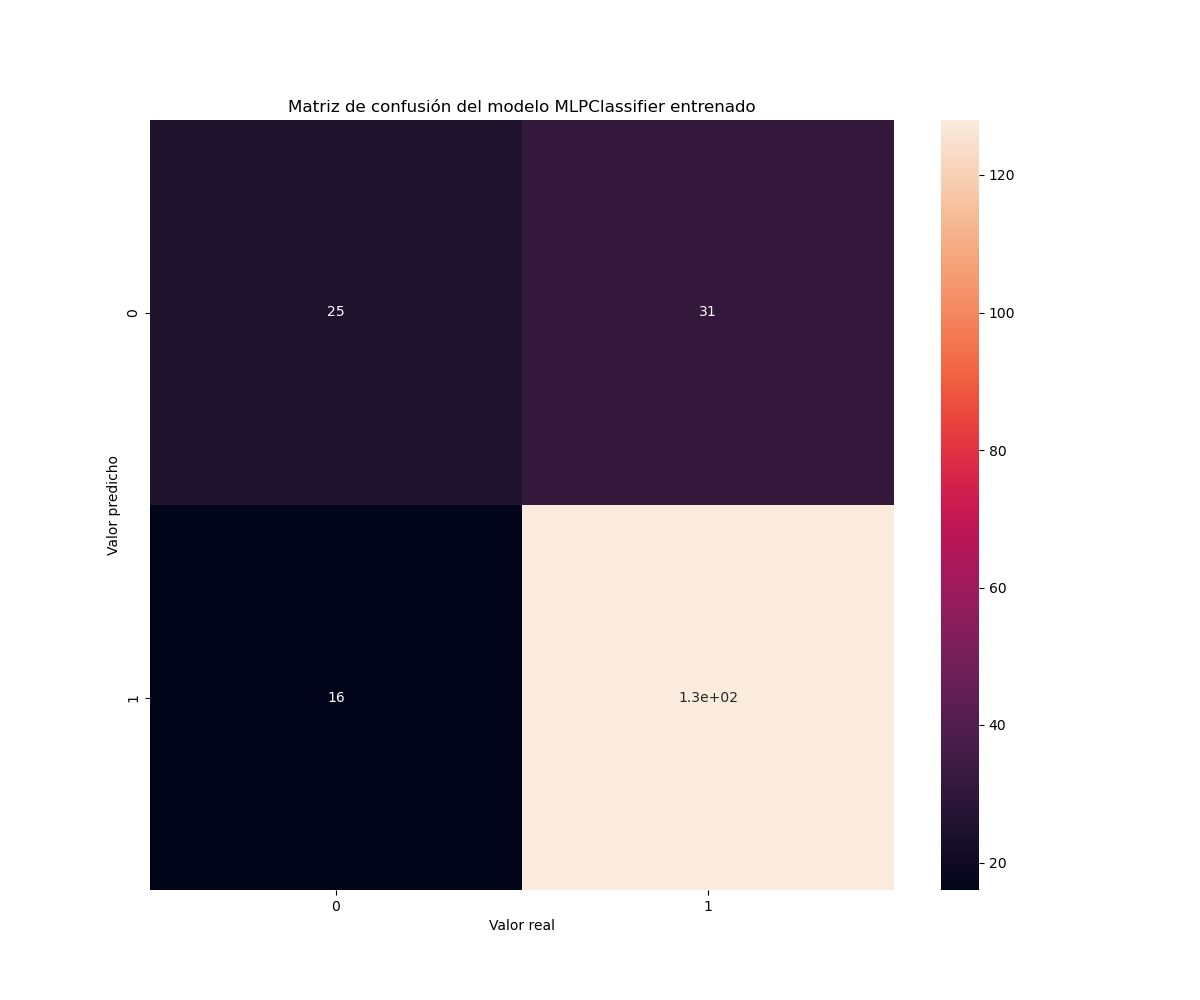
\includegraphics[scale = 0.6]{matriz_confusion_mejor.png}
	\caption{Matriz de confusión para las predicciones del conjunto de test del mejor modelo obtenido.}
	\label{fig:matriz_confusion_mejor}
\end{figure}

Como esperabamos, tenemos muchos datos en los que realmente se había cumplido el pago, ya que el problema estaba desbalanceado, sin embargo si que tenemos un problema para predecir los datos que tienen un valor real de no pagado, ya que de 41 datos con valor real que no se ha cumplido los pagos se ha equivocado en 16, casi la mitad.
